\documentclass[journal]{./IEEE/IEEEtran}
\usepackage{cite,graphicx,amsmath,mathtools,caption,fixltx2e,multicol}

\newcommand{\SPTITLE}{Sign Me Up: An Android Sign Language Translator Using Convolutional Neural Networks }
\newcommand{\ADVISEE}{Carlos Miguel E. Canonizado}
\newcommand{\ADVISER}{Jaime M. Samaniego}

\newcommand{\BSCS}{Bachelor of Science in Computer Science}
\newcommand{\ICS}{Institute of Computer Science}
\newcommand{\UPLB}{University of the Philippines Los Ba\~{n}os}
\newcommand{\REMARK}{\thanks{Presented to the Faculty of the \ICS, \UPLB\
                             in partial fulfillment of the requirements
                             for the Degree of \BSCS}}
        
\markboth{CMSC 190 Special Problem, \ICS}{}
\title{\SPTITLE}
\author{\ADVISEE~and~\ADVISER%
\REMARK
}
%\pubid{\copyright~2006~ICS \UPLB}

%%%%%%%%%%%%%%%%%%%%%%%%%%%%%%%%%%%%%%%%%%%%%%%%%%%%%%%%%%%%%%%%%%%%%%%%%%

\begin{document}

% TITLE
\maketitle

% ABSTRACT
\begin{abstract}
Sign language is widely used by both the deaf and hearing community. However, there is still a lot of people who are not knowledgeable of sign language. There are limited translators available for public use which includes text to sign language and vice-versa. "Sign Me Up" is an Android application which is designed to translate sign language even offline. It uses convolutional neural networks to translate gestures from the user and a series of reference images are provided for translating text to sign language. Through retraining the Inception-v3 model, the application gained the highest and lowest confidence levels of 97.8182\% and 27.1096\% respectively, affected by gestures similar to each other. An average of 60.0345\% confidence level was obtained for all gestures while averages of 81.9355\% and 97.4194\% for the top-1 and top-5 accuracies were obtained.
\end{abstract}

% INDEX TERMS
\begin{keywords}
android, sign language, neural network, convolution, convolutional neural network, inception model
\end{keywords}

% INTRODUCTION
\section{Introduction}

\subsection{Background of the Study}
Sign language is a system of communication that has been around for years. Its primary usage is to enable communication between the deaf and hearing people. The World Health Organization (WHO) \cite{WHO2018} estimated that by 2050, more than 900 million people will have disabling hearing loss. Given this large estimation, it is problematic that only a small percentage of people actually know how to use sign language. One of the most widely used sign language is the American Sign Language (ASL). The ASL gained its popularity after William Stokoe, Dorothy Casterline, and Carl Croneberg published their Dictionary of American Sign Language on Linguistic Principles in 1965 \cite{Wilcox1991}.
\newline
\indent When it comes to motion gesture technology, the earliest implementation was made possible through the use of gloves with sensors. Depending on the hand movement, signals were decoded by a computer by mapping a combination of signals to unique gestures \cite{Sharma2015}.  Today, technological advancements allow programmers to develop tools that deal with the likes of motion gesture recognition, without the use of any external equipment aside from cameras.
\newline
\indent Another technological advancement which will make this study feasible is the existence of Artificial Intelligence (AI). AI is a broad topic and one of its use many uses is the implementation of neural networks. A neural network is a set of connected processors or neurons which can be activated to produce a desired idea or result \cite{Schmidhuber2015}. Neural networks have different types but for image-related tasks, a convolutional neural network (CNN) is widely used due to its advantages for image classification or categorization \cite{Wu2016}.

\subsection{Objectives of the Study}
This study aims to develop an Android application to translate sign language. Specifically, this study intends to fulfill the following:

\begin{enumerate}
\item translate user inputted text to sign language using a series of image definitions;
\item translate user-captured sign language to text using convolutional neural networks; and
\item translate sign language regardless of the hand's orientation or size.
\end{enumerate}

\subsection{Significance of the Study}
\indent Being able to translate sign language to text or vice-versa will be beneficial not only for the deaf community but also for those who are aspiring to learn sign language. Moreover, the communication barrier between the deaf and non-deaf community will be minimized since they will have an accessible translator through this developed mobile application.
\newline
\indent Those who are trying to learn sign language will find the text to sign language useful while those who just want to translate sign language can simply use the sign language to text feature. Both of these features do not require any internet connectivity.
\newline
\indent In addition, most of the early sign language translators require the use of expensive devices such as smart gloves. Therefore, this application can be a cheaper alternative since smartphones are accessible and normal users can easily use the application without any additional setup. 

\subsection{Scope and Limitations of the Study}
\indent Given that sign language has many variations, it would be difficult to consider these variations all at once because of the existence of overlapping meanings among gestures. Thus, ASL was used as the standard vocabulary of this study to prevent ambiguities that may arise during implementation.
\newline
\indent Lastly, the data gathered was limited to the demographics of the University of the Philippines Los Ba\~{n}os area. Therefore, the model might not be able to translate hands of extremely light or dark complexion.
\newline

% RELATED LITERATURE
\section{Related Literature}
For several decades, understanding the deaf community has become a major challenge. Sign language, despite its many variations, is one of the most effective methods that allow the better communication between the deaf and the non-deaf community. Several studies have been conducted to further allow translation of sign language without actually learning the language.

\subsection{Previous Studies on Sign Language Translation}

\subsubsection{Support Vector Machine}
One implementation was done with the help of a Support Vector Machine (SVM). An SVM is used for analyzing data through classification, regression, and outliers detection. Additionally, an SVM is a supervised machine learning algorithm that is reliant on plotted data points. Villamor \cite{Villamor2018} was able to utilize an SVM in sign language translation through the following process: first, given an input image, the background and hand are identified. After that, the features of the hand are detected, examples of these features are the center of the palm, finger defect points, and finger vectors. These data are then plotted in an n-dimensional space, where n is the number of features. Once the points are plotted, the image is classified by finding the difference of two sets of points.
\newline
\subsubsection{Color Segmentation and Neural Networks} 
Another method that was used in translating sign language is color segmentation and neural networks. For this method, Akmeliawati \cite{Akmeliawati2007} used custom-made gloves to gather necessary data from the signer. Since there is a lot of unwanted data captured in an image or video, the frames were segmented according to the color that was visible in the gloves. This makes the translation easier since the program expects certain colors for each feature like yellow for the palm, purple for the thumb, red for the index and ring finger, and blue for the middle and pinky finger.
\newline
\indent This set-up produces data which are called vectors. A vector is a collection of numbers and for each finger, there is one xyvector giving a total of five xyvectors per hand. The weights of the data from these vectors are then fed into a neural network, to be specific, an artificial neural network (ANN). The ANN that Akmeliawati used had three neural networks: one for recognizing the alphabet, another for numbers, and the third one for word signs. After traversing these layers, a value will be returned if ever the ANN correctly classifies the input gesture. The use of color segmentation and ANN allowed Akmeliawati to detect dynamic signs such as fingerspelling.
\newline
\subsubsection{3D Trajectory Matching with Kinect}
Chai \cite{Chai} utilized Kinect by using its hand tracking technology. Through the hand tracking, a 3D trajectory was obtained which was then normalized through linear resampling. Normalization was done due to the differences in hand motion speed. After that, an existing gallery trajectory was used for the existing definitions and the input trajectory was aligned to get the recognition result.
\subsection{Convolutional Neural Network}
Convolutional neural networks (CNNs) are similar to traditional neural networks in the sense that they are comprised of neurons that are optimized through learning. Each node or neuron will still receive an input and perform activation functions. The main difference is that CNNs are primarily used for pattern recognition with images \cite{OShea2015}.
\newline
\indent O'Shea \cite{OShea2015} states that one of the largest limitations of regular neural networks is the lack of computational power required to compute data from images. Handwritten digits can be viable in regular neural networks since the image dimensions could be as small as 28 x 28. However, if we take a larger colored image input of 64 x 64, then the number of neurons for the first layer increases to an overwhelmingly large number of 12,288.
\newline 
\indent With traditional neural networks, there is a minimum of three layers: the input, output, and hidden layers in between. In CNN, there are additional layers namely: convolutional layer, pooling layer, and fully-connected layers. The process of recognizing an image in CNN is done by passing an input image to the input layer. The input layer will hold the pixel values of the image. Next, the convolutional layer will compute for the output of the neurons. The output is then passed to the pooling layer which will reduce the number of activation parameters by downsampling through a rectified linear unit (ReLu). This allows images of higher resolutions to be processed. After that, the fully-connected layers will attempt to produce a probability classification of each class.
\newline
\indent
The classification of high resolution images using convolutional neural network was emphasized in a study conducted by Krizhevsky \cite{Krizhevsky2012}. His deep convolutional network was trained to classify 1.2 million high-resolution images in the ImageNet LSVRC-2010 contest. The model had a top-1 error rate of 37.5 percent and a top-5 error rate of 17 percent.

\subsection{TensorFlow and Inception-v3}
TensorFlow is an open source platform for machine learning created by Google. It provides a diverse selection of models to use for free, and one of them is the Inception-v3 model. This model is a convolutional neural network trained for the ImageNet Large Visual Recognition Challenge using data from 2012 \cite{Szegedy2014}.
\newline
\indent The model produced a top-5 error rate of 3.46 percent. Its architecture can be seen below:

\begin{figure}[ht!]
    \centering
    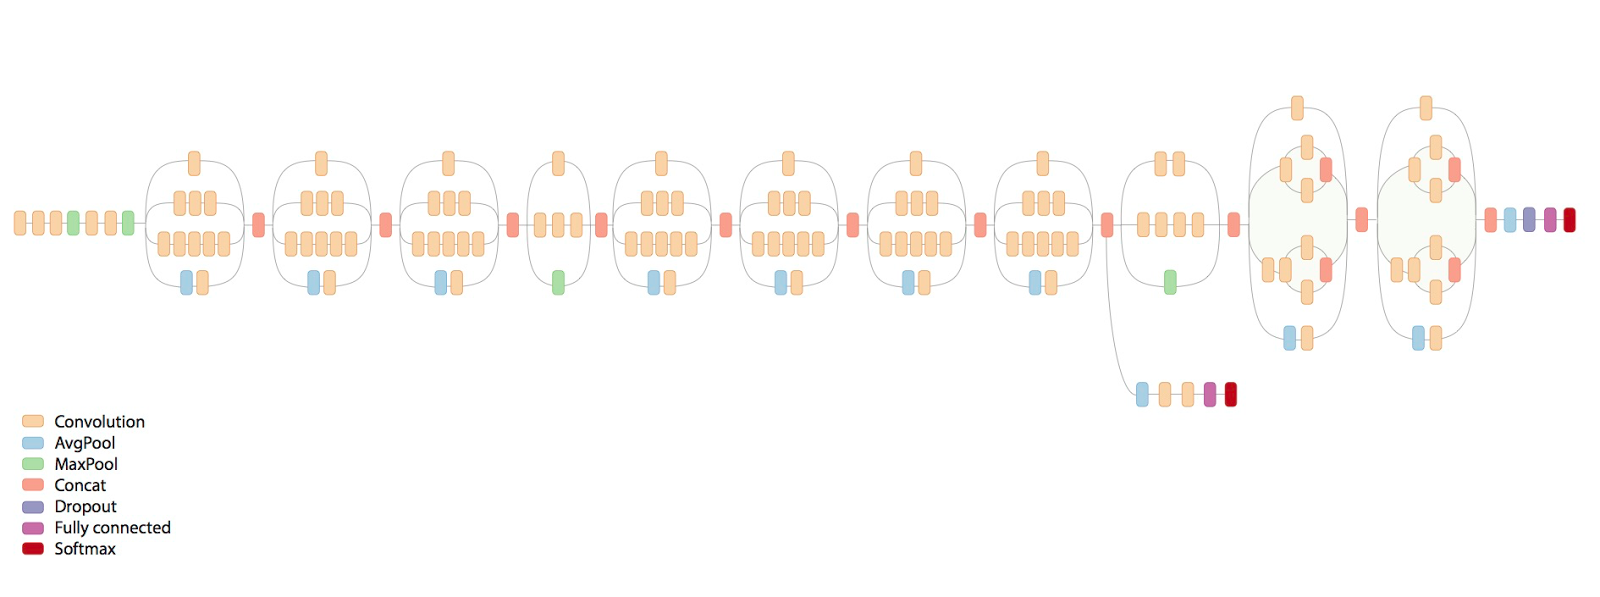
\includegraphics[width=1\linewidth]{./images/inception.png}
    \caption{Inception-v3 Architecture}
    \label{fig:inception}
\end{figure}

\indent With a model available such as Inception-v3, retraining can be done to modify its bottlenecks and create unique classifications such as sign language translation.

% METHODOLOGY
\section{Methodology}

\subsection{System Requirements}
The following were used used to develop the Android application:

\begin{itemize}
    \item A smartphone running on Android version 5.1.1 or higher for running the application;
    \item Android Studio version 3.2.1 or higher for creating the application;
    \item Python 3.7.1 for using scripts in model training;
    \item Conda 4.5.12 for creating a virtual environment for TensorFlow; and
    \item TensorFlow version 1.0 for the Inception-v3 retraining.
\end{itemize}

\subsection{Android Application}
The Android application is named "Sign Me Up''. It has two functionalities: one for translating sign language to text, and another for translating text to sign language. The home screen along with the icon of the application can be seen in Figure \ref{fig:home}:

\begin{figure}[ht!]
    \centering
    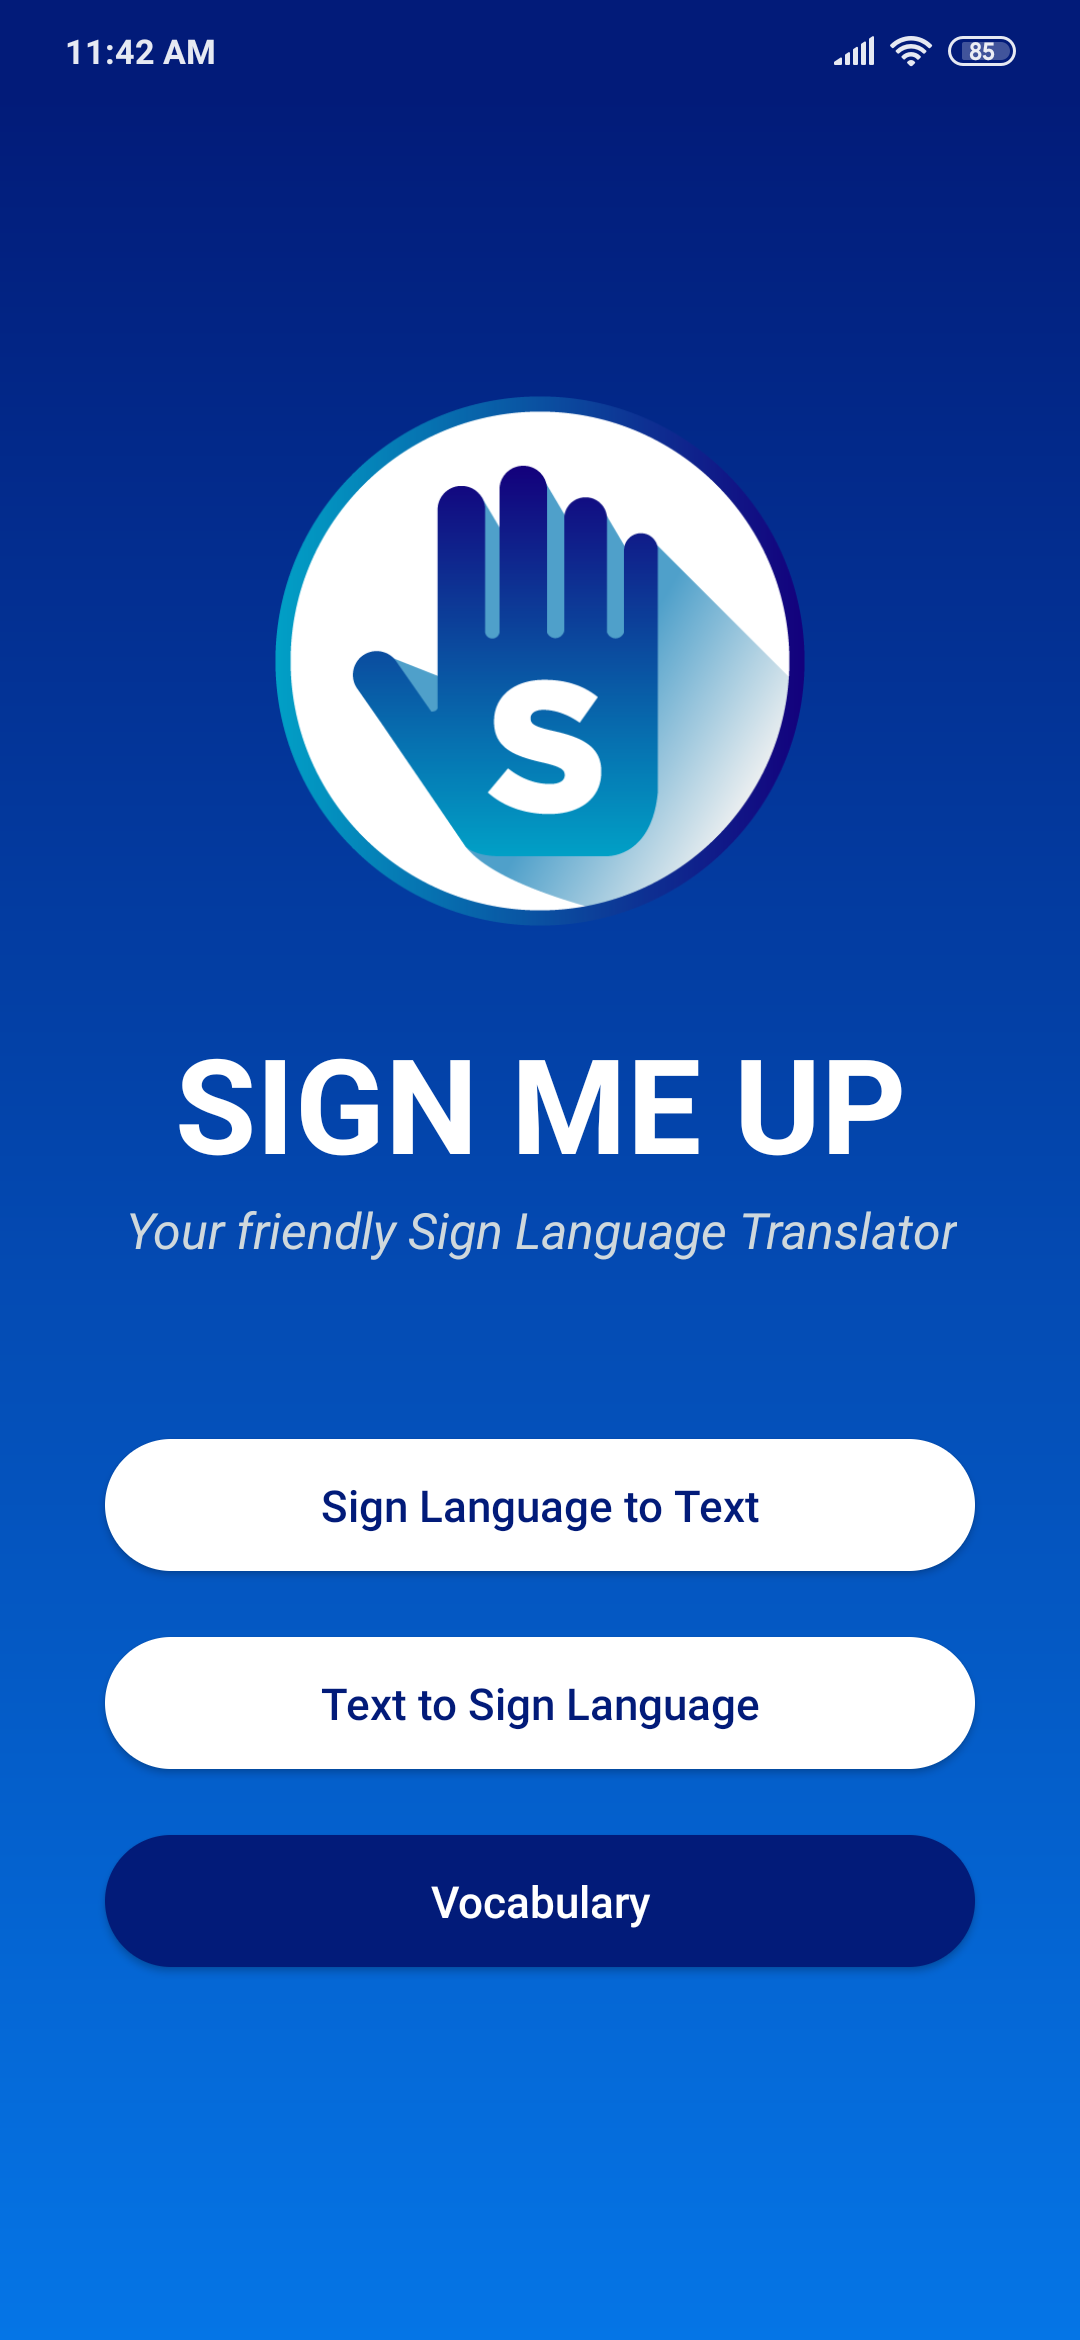
\includegraphics[width=0.75\linewidth]{./images/screen_home.png}
    \caption{Home Screen}
    \label{fig:home}
\end{figure}

\subsection{Vocabulary}
A total of 50 definitions were used. However, all the definitions are only available in text to sign language and a subset was used for sign language to text. The vocabulary can be seen in Figure \ref{fig:vocabulary}. 

\begin{figure}[ht!]
    \centering
    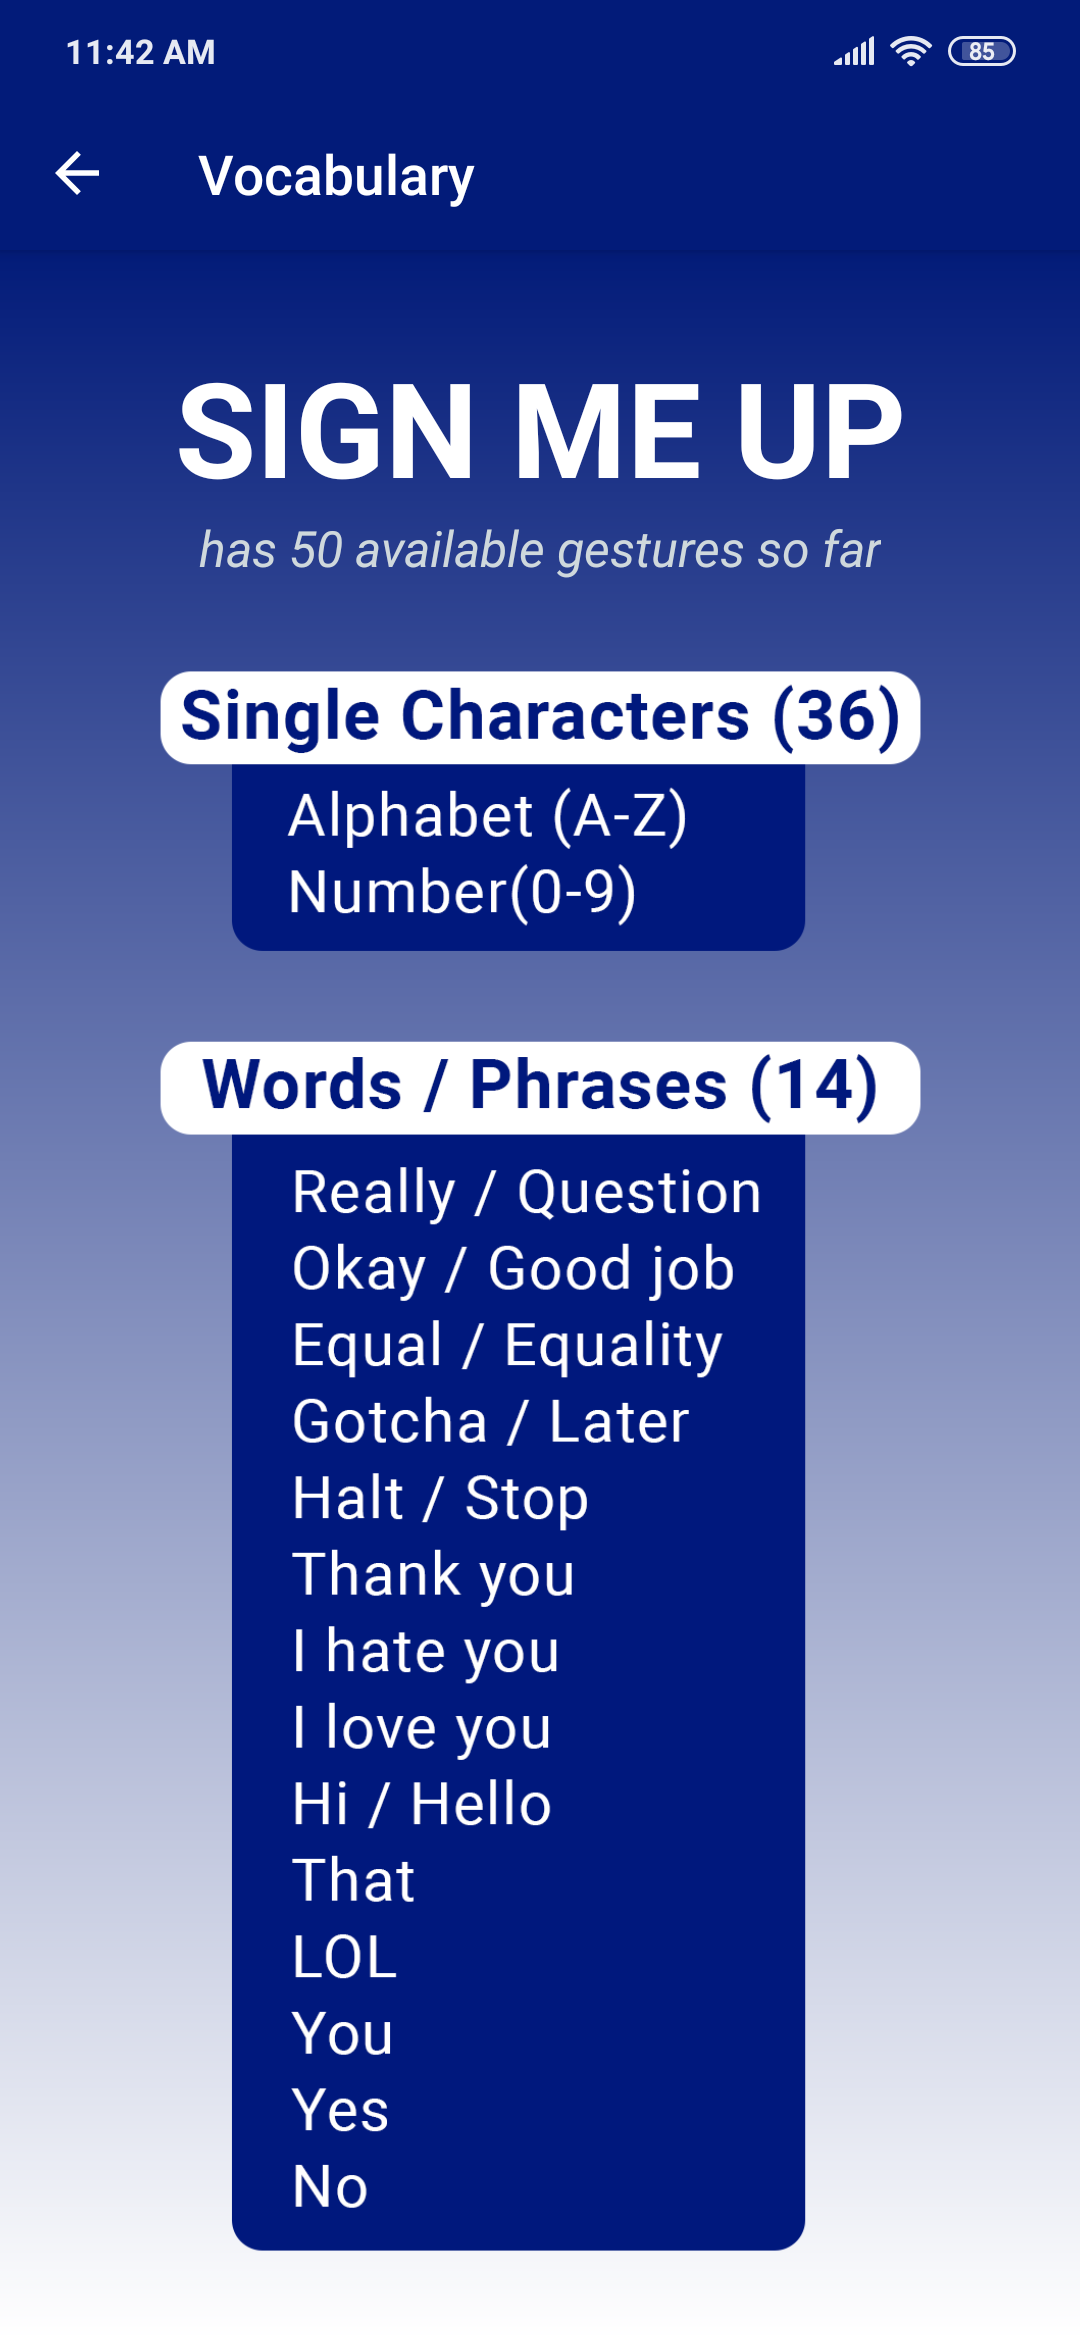
\includegraphics[width=0.75\linewidth]{./images/screen_vocabulary.png}
    \caption{Vocabulary Screen}
    \label{fig:vocabulary}
\end{figure}

\subsection{Data Gathering}
All data were gathered from random people in the University of the Philippines Los Ba\~{n}os. In sign language to text, only a subset of the vocabulary was used. These definitions are: the \textit{alphabet, yes, no, that, hi/hello,} and \textit{okay/good job} for a total of 31 gestures. Sample data is shown in Figure \ref{fig:data}.
\newline
\indent For every gesture, 40 people's hands were captured. The skin tone of the respondents were mostly fair to tan. All images were then flipped to cover the left and right-handed gestures, which added up to 80 pictures per gesture --- with a total of 2,480 data.
\newline
\indent The specifications of the camera used in data gathering can be found in Table I.

\begin{table}[ht!]
\centering
\caption{Camera Specifications}
\begin{tabular}{|l|l|}
\hline
\textbf{Model}            & OPPO A37           \\ \hline
\textbf{Camera}           & 8 MP               \\ \hline
\textbf{Image Resolution} & 2448 x 2448 Pixels \\ \hline
\end{tabular}
\end{table}

\begin{figure}[ht!]
    \centering
    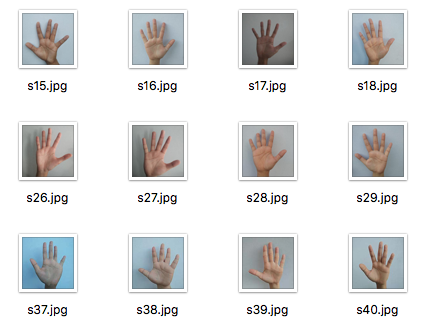
\includegraphics[width=1\linewidth]{./images/data.png}
    \caption{Sample Data}
    \label{fig:data}
\end{figure}

\subsection{Text to Sign Language}
The definitions available were mapped to a single reference photo. If the gesture involves movement, then the picture has a silhouette of a moving hand.
\newline
\indent Every input is checked to see if there are special characters. If there are any, the application will simply return an error message. Otherwise, the output will produce a series of images depending on the input of the user. It will first check if the input exists in the words available, if not, the words will be spelled out. Sample outputs can be seen in Figure \ref{fig:tts_result} and Figure \ref{fig:tts_error}.

\begin{figure}[ht!]
    \centering
    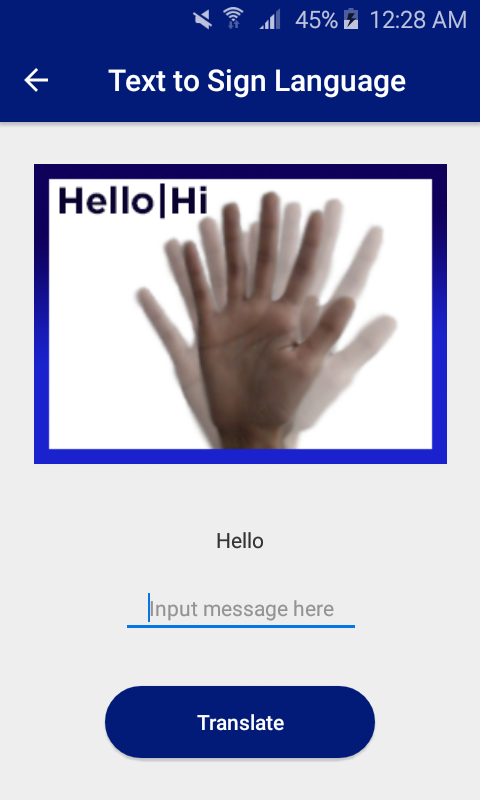
\includegraphics[width=0.75\linewidth]{./images/screen_tts_result.png}
    \caption{Sample Result}
    \label{fig:tts_result}
\end{figure}

\begin{figure}[ht!]
    \centering
    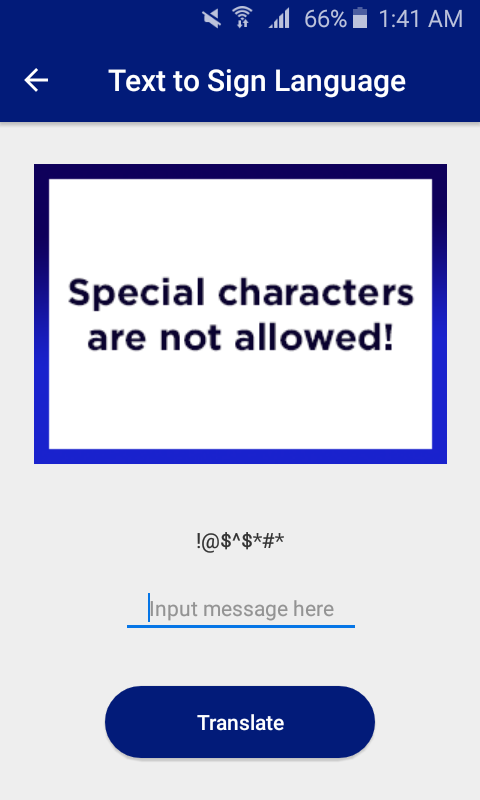
\includegraphics[width=0.75\linewidth]{./images/screen_tts_error.png}
    \caption{Invalid Input}
    \label{fig:tts_error}
\end{figure}


\subsection{Sign Language to Text}
\subsubsection{Retraining Inception-v3}
In order to classify the gestures, a convolutional neural network was used. Specifically, Inception-v3 was retrained so that the labels produced by the model are the definitions available for translation.
\newline
\indent This process is called transfer learning. From the old top/results layer of Inception-v3, a new layer was trained using the data gathered to fit the pretrained model. Out of the 2,480 data with 80 images per gesture, only 75 images per gesture were used for the training and validation. The remaining five images per gesture were used for testing.
\newline
\indent For the training itself, a total of 8000 epochs or training steps with a learning rate of 1 percent was used.
\newline
\subsubsection{Loading the Model in the Application}
Before using the model, it was optimized to reduce the pre-processing of the application and to reduce the size of the package. But optimizing was not enough because the size of the model was too big and unsuitable for mobile phones. This issue was addressed by quantizing the optimized model.
\newline
\indent Quantization was needed since majority of the space taken up by the model/output graph is from the weights or the large blocks of floating point numbers. Quantizing the weight of the networks helped in reducing the model's size. After this, the model was then loaded in the Android application.
\newline
\subsubsection{Getting Input}
The application's sign-to text feature primarily relies on the device having a camera. Once the user chooses to translate sign language to text, the camera will open and with a click of the translate button, the device will capture the image and it will feed it into the model.
\newline
\subsubsection{Showing Results}
When the model is done processing the image, the definition with the highest confidence level that is above the required threshold will be shown right above the translate button.
\newline
\indent After testing for the appropriate threshold, a minimum confidence level of 25 percent is required for a result to be returned to give way for similar gestures such as the letter c and o (see Figure \ref{fig:c_sample}). Anything less than that will not return anything as the model will most likely predict it as an invalid gesture. A reset button is also provided for clearing the output text. A successful run can be seen in Figures \ref{fig:stt_initial} and \ref{fig:stt_result}.

\begin{figure}[ht!]
    \centering
    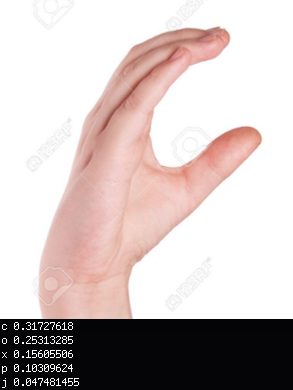
\includegraphics[width=1\linewidth]{./images/c_sample.png}
    \caption{31.72\% letter c (CORRECT)}
    \label{fig:c_sample}
\end{figure}

\begin{figure}[ht!]
    \centering
    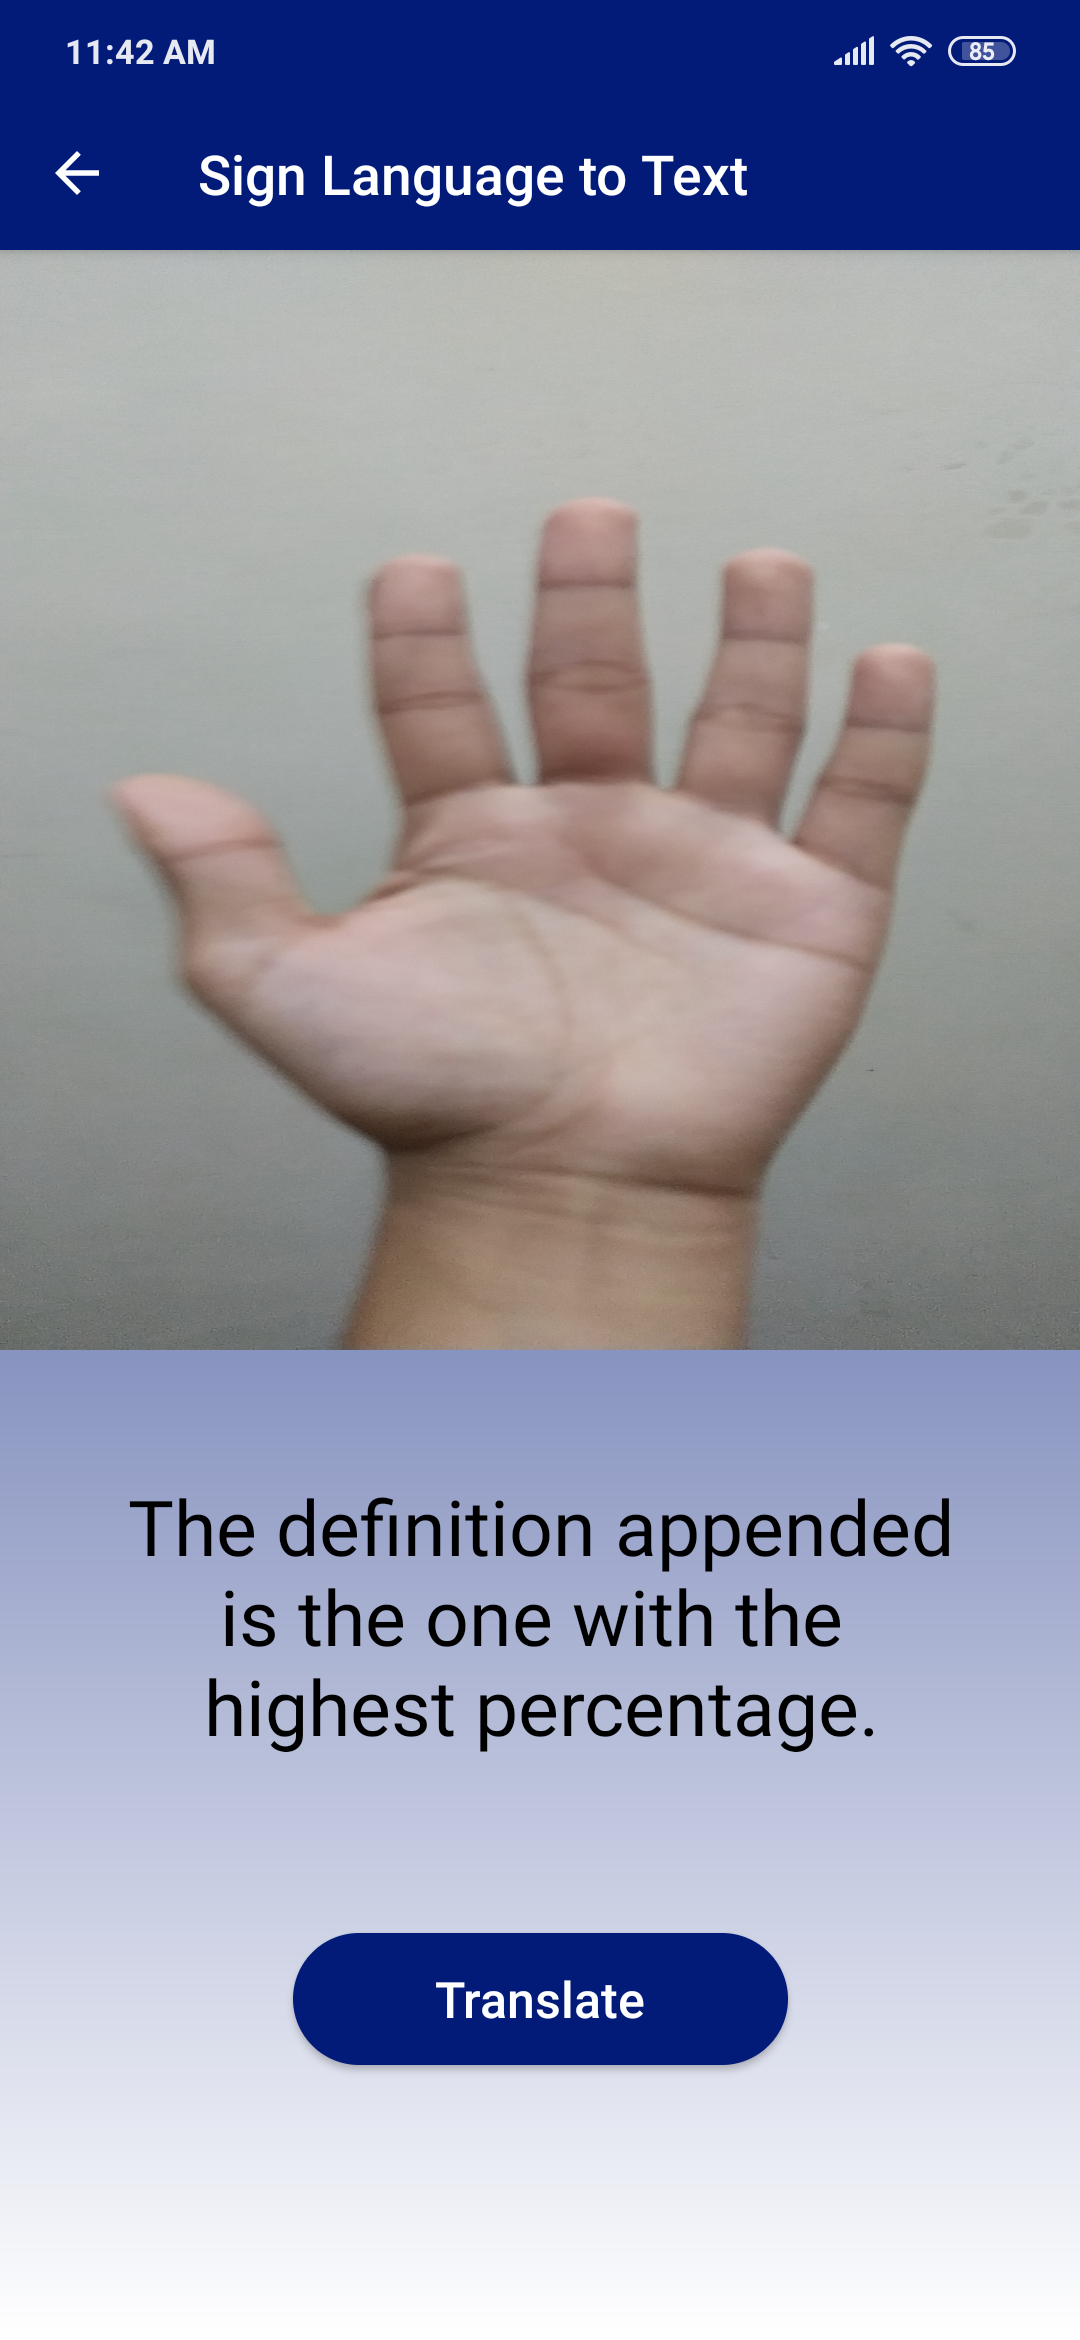
\includegraphics[width=1\linewidth]{./images/screen_stt_initial.png}
    \caption{Left to Right: Initial and Translating Screens}
    \label{fig:stt_initial}
\end{figure}

\begin{figure}[ht!]
    \centering
    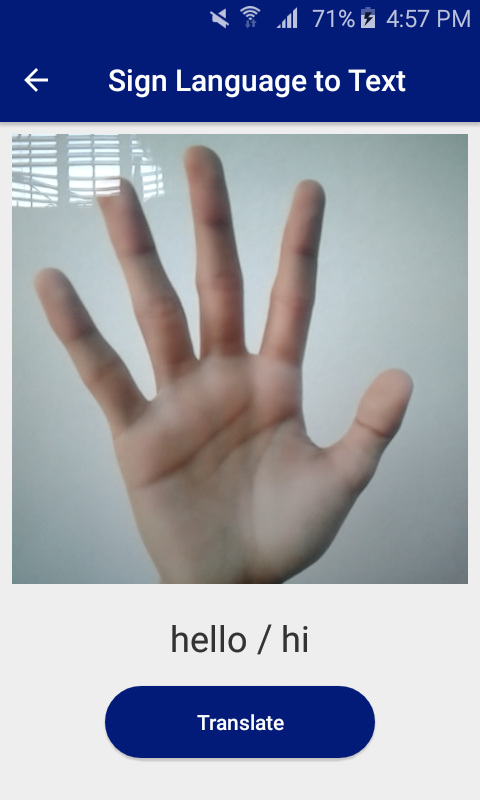
\includegraphics[width=0.75\linewidth]{./images/screen_stt_result.png}
    \caption{Result Screen}
    \label{fig:stt_result}
\end{figure}


\subsection{Evaluation}
The results from the tests were measured and evaluated with the following metrics:
\begin{enumerate}
    \item \textit{Confidence level} - refers to the certainty of the model's prediction.
    \item \textit{Top-1 accuracy rate} - determines the rate at which the gesture was translated correctly.
    \item \textit{Top-5 accuracy rate} - notes how often the target label was predicted within the five most probable guesses.
\end{enumerate}


% RESULTS AND DISCUSSION
\section{Results and Discussion}

Out of the 2,480 data, five images per gesture were taken to test the accuracy of the model. Table II shows the mean confidence level during the testing phase, along with the top-1 and top-5 accuracy rates (in percentages).

\begin{table}[ht!]
\centering
\caption{Results from testing five images per gesture}
\begin{tabular}{|l|c|c|c|}
\hline
\multicolumn{1}{|c|}{\textbf{Gesture}} & \textbf{Confidence} & \textbf{Top-1 Accuracy} & \textbf{Top-5 Accuracy} \\ \hline
a                                      & 62.4498                   & 80                      & 80                      \\ \hline
b                                      & 27.1096                   & 20                      & 100                     \\ \hline
c                                      & 91.5403                   & 100                     & 100                     \\ \hline
d                                      & 75.4884                   & 100                     & 100                     \\ \hline
e                                      & 71.3239                   & 100                     & 100                     \\ \hline
f                                      & 69.2242                   & 100                     & 100                     \\ \hline
g                                      & 47.1842                   & 80                      & 100                     \\ \hline
h                                      & 88.2374                   & 100                     & 100                     \\ \hline
hello/hi                             & 71.6996                   & 100                     & 100                     \\ \hline
i                                      & 71.6996                   & 60                      & 80                      \\ \hline
j                                      & 57.5536                   & 80                      & 100                     \\ \hline
k                                      & 38.9782                   & 60                      & 100                     \\ \hline
l                                      & 73.5850                   & 100                     & 100                     \\ \hline
m                                      & 35.2467                   & 60                      & 100                     \\ \hline
n                                      & 55.8013                   & 80                      & 100                     \\ \hline
no                                     & 58.3989                   & 80                      & 100                     \\ \hline
o                                      & 79.4044                   & 100                     & 100                     \\ \hline
okay/good job                        & 97.8182                   & 100                     & 100                     \\ \hline
p                                      & 75.8770                   & 100                     & 100                     \\ \hline
q                                      & 45.2842                   & 60                      & 100                     \\ \hline
r                                      & 43.0818                   & 100                     & 100                     \\ \hline
s                                      & 56.6103                   & 80                      & 100                     \\ \hline
t                                      & 34.6972                   & 60                      & 60                      \\ \hline
that                                   & 78.4250                   & 80                      & 100                     \\ \hline
u                                      & 57.2008                   & 80                      & 100                     \\ \hline
v                                      & 55.1236                   & 80                      & 100                     \\ \hline
w                                      & 66.2519                   & 80                      & 100                     \\ \hline
x                                      & 39.9979                   & 80                      & 100                     \\ \hline
y                                      & 73.9857                   & 80                      & 100                     \\ \hline
yes                                    & 58.3642                   & 80                      & 100                     \\ \hline
z                                      & 42.2726                   & 80                      & 100                     \\ \hline
\end{tabular}
\end{table}

\indent An average of 60.0345\% confidence level was obtained for all gestures while averages of 81.9355\% and 97.4194\% for the top-1 and top-5 accuracies were obtained.
\newline
\indent Gestures with low confidence level do not necessarily entail that the model fails to correctly classify them. Since most of the features of the hands are similar, gestures that look like one another can affect the confidence levels. An example can be seen in Figure \ref{fig:wrong_results} where the predictions for m and n were switched. 

\begin{figure}[ht!]
    \centering
    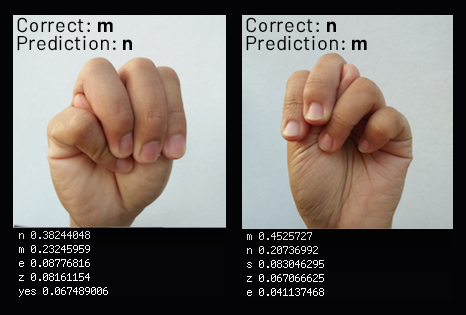
\includegraphics[width=1\linewidth]{./images/wrong_results.png}
    \caption{Left to Right: m classified as n and n classified as m}
    \label{fig:wrong_results}
\end{figure}

\indent \textit{Okay/good job} is the gesture with the highest confidence level (97.8182\%) since it is the most unique gesture out of the 31 available. Meanwhile, the gesture with the lowest confidence level is \textit{b} with 27.1096\%. The more the gestures have similarities, the lower the produced confidence level will be since the probability will be distributed. Although with similar gestures, they can still be classified correctly according to the top-1 accuracy rates. If not, then the target label is still part of the top-5 predictions.
\newline
\indent There were gestures with perfect predictions, namely: \textit{c, d, e, f, h, hello/hi, l, o, okay/good job, p,} and \textit{r}. However, this does not guarantee that the model will be able to perfectly predict these gestures all the time. The gestures which produced inaccurate predictions can be found in Table III along with the gestures they were confused with.

\begin{table}[ht!]
\centering
\caption{Wrong predictions - these predictions happened at most one time except for b = f which occurred two times out of five test cases}
\begin{tabular}{|l|l|}
\hline
\multicolumn{1}{|c|}{\textbf{Gesture}} & \multicolumn{1}{c|}{\textbf{Wrong Predictions}}         \\ \hline
a                                      & - s                                                     \\ \hline
b                                      & \begin{tabular}[c]{@{}l@{}}- f\\ - k\\ - v\end{tabular} \\ \hline
g                                      & - h                                                     \\ \hline
i                                      & \begin{tabular}[c]{@{}l@{}}- f\\ - n\end{tabular}       \\ \hline
j                                      & - h                                                     \\ \hline
k                                      & \begin{tabular}[c]{@{}l@{}}- v\\ - w\end{tabular}       \\ \hline
m                                      & \begin{tabular}[c]{@{}l@{}}- i\\ - n\end{tabular}       \\ \hline
n                                      & - m                                                     \\ \hline
no                                     & - z                                                     \\ \hline
q                                      & \begin{tabular}[c]{@{}l@{}}- o\\ - x\end{tabular}       \\ \hline
s                                      & - n                                                     \\ \hline
t                                      & \begin{tabular}[c]{@{}l@{}}- y\\ - o\end{tabular}       \\ \hline
that                                   & - y                                                     \\ \hline
u                                      & - r                                                     \\ \hline
v                                      & - w                                                     \\ \hline
w                                      & - v                                                     \\ \hline
x                                      & - v                                                     \\ \hline
y                                      & - n                                                     \\ \hline
yes                                    & - a                                                     \\ \hline
z                                      & - r                                                     \\ \hline
\end{tabular}
\end{table}

% CONCLUSION
\section{Conclusion}
Translating sign language to text using convolutional neural networks is a feasible approach. It is powerful and compared to other neural networks, it can work with high resolution images. However, a significant amount of training data is needed to make the model more accurate. Further optimization is also required to speed up the sign language to text feature. Detecting moving gestures was not achieved aside from looking at the most significant frame due to the delays of retrieving the predictions. 

% RECOMMENDATION
\section{Recommendation}
One of the biggest challenges in implementing sign language translators is the translation of moving gestures. If the application could be optimized more so that the capturing of the images and returning of the results are faster, then the frames can be chained to check if the gesture being done is correct. Otherwise, another approach or model may be more appropriate in solving this issue. Other rooms for improvement are as follows:
\newline
\subsubsection{Data Gathering}
It is highly recommended to have a larger data set when retraining the model. As much as possible, try to consider different skin tones and hand sizes. To add, be more strict with the lighting conditions and minimize shadows. Make sure that the signer knows the correct form and make the gestures uniform with little to no differences.
\newline
\subsubsection{Model Optimization}
Even with the optimization methods done in this study, the model can be made lighter if emerging technologies such as TensorFlow Lite, are used. Models built for mobile applications such as MobileNet can also be used for faster results.
\newline
\subsubsection{Interface}
Redesign the other screens to make it more appealing. Allowing the user to turn on the phone's torch without going through the phone's settings could be useful while translating sign language to text.

% BIBLIOGRAPHY
\bibliographystyle{./IEEE/IEEEtran}
\bibliography{./cs190}

\end{document}
 
